\documentclass[12pt]{article}\usepackage{graphicx, color}
%% maxwidth is the original width if it is less than linewidth
%% otherwise use linewidth (to make sure the graphics do not exceed the margin)
\makeatletter
\def\maxwidth{ %
  \ifdim\Gin@nat@width>\linewidth
    \linewidth
  \else
    \Gin@nat@width
  \fi
}
\makeatother

\definecolor{fgcolor}{rgb}{0.2, 0.2, 0.2}
\newcommand{\hlnumber}[1]{\textcolor[rgb]{0,0,0}{#1}}%
\newcommand{\hlfunctioncall}[1]{\textcolor[rgb]{0.501960784313725,0,0.329411764705882}{\textbf{#1}}}%
\newcommand{\hlstring}[1]{\textcolor[rgb]{0.6,0.6,1}{#1}}%
\newcommand{\hlkeyword}[1]{\textcolor[rgb]{0,0,0}{\textbf{#1}}}%
\newcommand{\hlargument}[1]{\textcolor[rgb]{0.690196078431373,0.250980392156863,0.0196078431372549}{#1}}%
\newcommand{\hlcomment}[1]{\textcolor[rgb]{0.180392156862745,0.6,0.341176470588235}{#1}}%
\newcommand{\hlroxygencomment}[1]{\textcolor[rgb]{0.43921568627451,0.47843137254902,0.701960784313725}{#1}}%
\newcommand{\hlformalargs}[1]{\textcolor[rgb]{0.690196078431373,0.250980392156863,0.0196078431372549}{#1}}%
\newcommand{\hleqformalargs}[1]{\textcolor[rgb]{0.690196078431373,0.250980392156863,0.0196078431372549}{#1}}%
\newcommand{\hlassignement}[1]{\textcolor[rgb]{0,0,0}{\textbf{#1}}}%
\newcommand{\hlpackage}[1]{\textcolor[rgb]{0.588235294117647,0.709803921568627,0.145098039215686}{#1}}%
\newcommand{\hlslot}[1]{\textit{#1}}%
\newcommand{\hlsymbol}[1]{\textcolor[rgb]{0,0,0}{#1}}%
\newcommand{\hlprompt}[1]{\textcolor[rgb]{0.2,0.2,0.2}{#1}}%

\usepackage{framed}
\makeatletter
\newenvironment{kframe}{%
 \def\at@end@of@kframe{}%
 \ifinner\ifhmode%
  \def\at@end@of@kframe{\end{minipage}}%
  \begin{minipage}{\columnwidth}%
 \fi\fi%
 \def\FrameCommand##1{\hskip\@totalleftmargin \hskip-\fboxsep
 \colorbox{shadecolor}{##1}\hskip-\fboxsep
     % There is no \\@totalrightmargin, so:
     \hskip-\linewidth \hskip-\@totalleftmargin \hskip\columnwidth}%
 \MakeFramed {\advance\hsize-\width
   \@totalleftmargin\z@ \linewidth\hsize
   \@setminipage}}%
 {\par\unskip\endMakeFramed%
 \at@end@of@kframe}
\makeatother

\definecolor{shadecolor}{rgb}{.97, .97, .97}
\definecolor{messagecolor}{rgb}{0, 0, 0}
\definecolor{warningcolor}{rgb}{1, 0, 1}
\definecolor{errorcolor}{rgb}{1, 0, 0}
\newenvironment{knitrout}{}{} % an empty environment to be redefined in TeX

\usepackage{alltt}
\usepackage{tikz}
\usepackage{tipa}
\usepackage[hmargin=1.54cm,vmargin=1.54cm]{geometry}
\geometry{a4paper}
\usepackage{fancyhdr} % This should be set AFTER setting up the page geometry
\pagestyle{fancy} % options: empty , plain , fancy
\renewcommand{\headrulewidth}{0pt} % customise the layout...
\lhead{}\chead{}\rhead{}
\lfoot{}\cfoot{}\rfoot{}
\IfFileExists{upquote.sty}{\usepackage{upquote}}{}




\begin{document}













\begin{knitrout}
\definecolor{shadecolor}{rgb}{0.969, 0.969, 0.969}\color{fgcolor}\begin{kframe}


{\ttfamily\noindent\bfseries\color{errorcolor}{\#\# Error: Cannot create:\\\#\# 	 /Users/casillas/Desktop/master/plots\_folder/cars-plot.tex \\\#\# Because the directory does not exist or is not writable.}}\end{kframe}
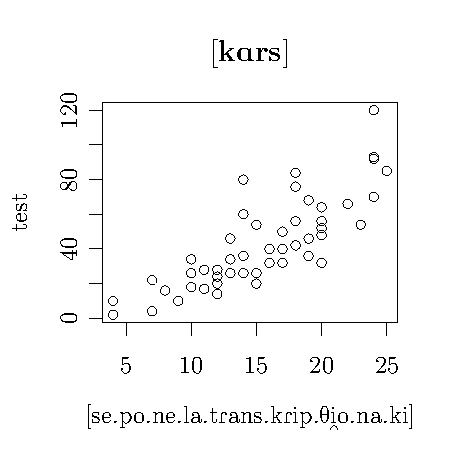
\includegraphics[width=\maxwidth]{figure/cars} 

\end{knitrout}


\begin{figure}
\caption{Here is the cars plot}
\centering
% Created by tikzDevice version 0.6.2 on 2013-05-17 11:59:32
% !TEX encoding = UTF-8 Unicode
\begin{tikzpicture}[x=1pt,y=1pt]
\definecolor[named]{drawColor}{rgb}{0.00,0.00,0.00}
\definecolor[named]{fillColor}{rgb}{1.00,1.00,1.00}
\fill[color=fillColor,fill opacity=0.00,] (0,0) rectangle (505.89,505.89);
\begin{scope}
\path[clip] ( 49.20, 61.20) rectangle (480.69,456.69);
\definecolor[named]{drawColor}{rgb}{0.00,0.00,0.00}

\draw[color=drawColor,line cap=round,line join=round,fill opacity=0.00,] ( 65.18, 75.85) circle (  2.25);

\draw[color=drawColor,line cap=round,line join=round,fill opacity=0.00,] ( 65.18,100.67) circle (  2.25);

\draw[color=drawColor,line cap=round,line join=round,fill opacity=0.00,] (122.26, 82.05) circle (  2.25);

\draw[color=drawColor,line cap=round,line join=round,fill opacity=0.00,] (122.26,137.91) circle (  2.25);

\draw[color=drawColor,line cap=round,line join=round,fill opacity=0.00,] (141.28,119.29) circle (  2.25);

\draw[color=drawColor,line cap=round,line join=round,fill opacity=0.00,] (160.31,100.67) circle (  2.25);

\draw[color=drawColor,line cap=round,line join=round,fill opacity=0.00,] (179.33,125.50) circle (  2.25);

\draw[color=drawColor,line cap=round,line join=round,fill opacity=0.00,] (179.33,150.33) circle (  2.25);

\draw[color=drawColor,line cap=round,line join=round,fill opacity=0.00,] (179.33,175.15) circle (  2.25);

\draw[color=drawColor,line cap=round,line join=round,fill opacity=0.00,] (198.36,122.40) circle (  2.25);

\draw[color=drawColor,line cap=round,line join=round,fill opacity=0.00,] (198.36,156.53) circle (  2.25);

\draw[color=drawColor,line cap=round,line join=round,fill opacity=0.00,] (217.38,113.09) circle (  2.25);

\draw[color=drawColor,line cap=round,line join=round,fill opacity=0.00,] (217.38,131.71) circle (  2.25);

\draw[color=drawColor,line cap=round,line join=round,fill opacity=0.00,] (217.38,144.12) circle (  2.25);

\draw[color=drawColor,line cap=round,line join=round,fill opacity=0.00,] (217.38,156.53) circle (  2.25);

\draw[color=drawColor,line cap=round,line join=round,fill opacity=0.00,] (236.41,150.33) circle (  2.25);

\draw[color=drawColor,line cap=round,line join=round,fill opacity=0.00,] (236.41,175.15) circle (  2.25);

\draw[color=drawColor,line cap=round,line join=round,fill opacity=0.00,] (236.41,175.15) circle (  2.25);

\draw[color=drawColor,line cap=round,line join=round,fill opacity=0.00,] (236.41,212.39) circle (  2.25);

\draw[color=drawColor,line cap=round,line join=round,fill opacity=0.00,] (255.43,150.33) circle (  2.25);

\draw[color=drawColor,line cap=round,line join=round,fill opacity=0.00,] (255.43,181.36) circle (  2.25);

\draw[color=drawColor,line cap=round,line join=round,fill opacity=0.00,] (255.43,255.84) circle (  2.25);

\draw[color=drawColor,line cap=round,line join=round,fill opacity=0.00,] (255.43,317.91) circle (  2.25);

\draw[color=drawColor,line cap=round,line join=round,fill opacity=0.00,] (274.46,131.71) circle (  2.25);

\draw[color=drawColor,line cap=round,line join=round,fill opacity=0.00,] (274.46,150.33) circle (  2.25);

\draw[color=drawColor,line cap=round,line join=round,fill opacity=0.00,] (274.46,237.22) circle (  2.25);

\draw[color=drawColor,line cap=round,line join=round,fill opacity=0.00,] (293.48,168.95) circle (  2.25);

\draw[color=drawColor,line cap=round,line join=round,fill opacity=0.00,] (293.48,193.77) circle (  2.25);

\draw[color=drawColor,line cap=round,line join=round,fill opacity=0.00,] (312.51,168.95) circle (  2.25);

\draw[color=drawColor,line cap=round,line join=round,fill opacity=0.00,] (312.51,193.77) circle (  2.25);

\draw[color=drawColor,line cap=round,line join=round,fill opacity=0.00,] (312.51,224.81) circle (  2.25);

\draw[color=drawColor,line cap=round,line join=round,fill opacity=0.00,] (331.53,199.98) circle (  2.25);

\draw[color=drawColor,line cap=round,line join=round,fill opacity=0.00,] (331.53,243.43) circle (  2.25);

\draw[color=drawColor,line cap=round,line join=round,fill opacity=0.00,] (331.53,305.50) circle (  2.25);

\draw[color=drawColor,line cap=round,line join=round,fill opacity=0.00,] (331.53,330.32) circle (  2.25);

\draw[color=drawColor,line cap=round,line join=round,fill opacity=0.00,] (350.56,181.36) circle (  2.25);

\draw[color=drawColor,line cap=round,line join=round,fill opacity=0.00,] (350.56,212.39) circle (  2.25);

\draw[color=drawColor,line cap=round,line join=round,fill opacity=0.00,] (350.56,280.67) circle (  2.25);

\draw[color=drawColor,line cap=round,line join=round,fill opacity=0.00,] (369.58,168.95) circle (  2.25);

\draw[color=drawColor,line cap=round,line join=round,fill opacity=0.00,] (369.58,218.60) circle (  2.25);

\draw[color=drawColor,line cap=round,line join=round,fill opacity=0.00,] (369.58,231.01) circle (  2.25);

\draw[color=drawColor,line cap=round,line join=round,fill opacity=0.00,] (369.58,243.43) circle (  2.25);

\draw[color=drawColor,line cap=round,line join=round,fill opacity=0.00,] (369.58,268.26) circle (  2.25);

\draw[color=drawColor,line cap=round,line join=round,fill opacity=0.00,] (407.63,274.46) circle (  2.25);

\draw[color=drawColor,line cap=round,line join=round,fill opacity=0.00,] (426.66,237.22) circle (  2.25);

\draw[color=drawColor,line cap=round,line join=round,fill opacity=0.00,] (445.68,286.88) circle (  2.25);

\draw[color=drawColor,line cap=round,line join=round,fill opacity=0.00,] (445.68,355.15) circle (  2.25);

\draw[color=drawColor,line cap=round,line join=round,fill opacity=0.00,] (445.68,358.25) circle (  2.25);

\draw[color=drawColor,line cap=round,line join=round,fill opacity=0.00,] (445.68,442.04) circle (  2.25);

\draw[color=drawColor,line cap=round,line join=round,fill opacity=0.00,] (464.71,333.43) circle (  2.25);
\end{scope}
\begin{scope}
\path[clip] (  0.00,  0.00) rectangle (505.89,505.89);
\definecolor[named]{drawColor}{rgb}{0.00,0.00,0.00}

\draw[color=drawColor,line cap=round,line join=round,fill opacity=0.00,] ( 84.21, 61.20) -- (464.71, 61.20);

\draw[color=drawColor,line cap=round,line join=round,fill opacity=0.00,] ( 84.21, 61.20) -- ( 84.21, 55.20);

\draw[color=drawColor,line cap=round,line join=round,fill opacity=0.00,] (179.33, 61.20) -- (179.33, 55.20);

\draw[color=drawColor,line cap=round,line join=round,fill opacity=0.00,] (274.46, 61.20) -- (274.46, 55.20);

\draw[color=drawColor,line cap=round,line join=round,fill opacity=0.00,] (369.58, 61.20) -- (369.58, 55.20);

\draw[color=drawColor,line cap=round,line join=round,fill opacity=0.00,] (464.71, 61.20) -- (464.71, 55.20);

\node[color=drawColor,anchor=base,inner sep=0pt, outer sep=0pt, scale=  1.00] at ( 84.21, 37.20) {5};

\node[color=drawColor,anchor=base,inner sep=0pt, outer sep=0pt, scale=  1.00] at (179.33, 37.20) {10};

\node[color=drawColor,anchor=base,inner sep=0pt, outer sep=0pt, scale=  1.00] at (274.46, 37.20) {15};

\node[color=drawColor,anchor=base,inner sep=0pt, outer sep=0pt, scale=  1.00] at (369.58, 37.20) {20};

\node[color=drawColor,anchor=base,inner sep=0pt, outer sep=0pt, scale=  1.00] at (464.71, 37.20) {25};

\draw[color=drawColor,line cap=round,line join=round,fill opacity=0.00,] ( 49.20, 69.64) -- ( 49.20,442.04);

\draw[color=drawColor,line cap=round,line join=round,fill opacity=0.00,] ( 49.20, 69.64) -- ( 43.20, 69.64);

\draw[color=drawColor,line cap=round,line join=round,fill opacity=0.00,] ( 49.20,131.71) -- ( 43.20,131.71);

\draw[color=drawColor,line cap=round,line join=round,fill opacity=0.00,] ( 49.20,193.77) -- ( 43.20,193.77);

\draw[color=drawColor,line cap=round,line join=round,fill opacity=0.00,] ( 49.20,255.84) -- ( 43.20,255.84);

\draw[color=drawColor,line cap=round,line join=round,fill opacity=0.00,] ( 49.20,317.91) -- ( 43.20,317.91);

\draw[color=drawColor,line cap=round,line join=round,fill opacity=0.00,] ( 49.20,379.98) -- ( 43.20,379.98);

\draw[color=drawColor,line cap=round,line join=round,fill opacity=0.00,] ( 49.20,442.04) -- ( 43.20,442.04);

\node[rotate= 90.00,color=drawColor,anchor=base,inner sep=0pt, outer sep=0pt, scale=  1.00] at ( 37.20, 69.64) {0};

\node[rotate= 90.00,color=drawColor,anchor=base,inner sep=0pt, outer sep=0pt, scale=  1.00] at ( 37.20,131.71) {20};

\node[rotate= 90.00,color=drawColor,anchor=base,inner sep=0pt, outer sep=0pt, scale=  1.00] at ( 37.20,193.77) {40};

\node[rotate= 90.00,color=drawColor,anchor=base,inner sep=0pt, outer sep=0pt, scale=  1.00] at ( 37.20,255.84) {60};

\node[rotate= 90.00,color=drawColor,anchor=base,inner sep=0pt, outer sep=0pt, scale=  1.00] at ( 37.20,317.91) {80};

\node[rotate= 90.00,color=drawColor,anchor=base,inner sep=0pt, outer sep=0pt, scale=  1.00] at ( 37.20,379.98) {100};

\node[rotate= 90.00,color=drawColor,anchor=base,inner sep=0pt, outer sep=0pt, scale=  1.00] at ( 37.20,442.04) {120};

\draw[color=drawColor,line cap=round,line join=round,fill opacity=0.00,] ( 49.20, 61.20) --
	(480.69, 61.20) --
	(480.69,456.69) --
	( 49.20,456.69) --
	( 49.20, 61.20);
\end{scope}
\begin{scope}
\path[clip] (  0.00,  0.00) rectangle (505.89,505.89);
\definecolor[named]{drawColor}{rgb}{0.00,0.00,0.00}

\node[color=drawColor,anchor=base,inner sep=0pt, outer sep=0pt, scale=  1.20] at (264.94,476.32) {\bfseries [\textipa{k}\textscripta rs]};

\node[color=drawColor,anchor=base,inner sep=0pt, outer sep=0pt, scale=  1.00] at (264.94, 13.20) {[se.po.ne.la.t\textipa{R}ans.k\textipa{R}ip.\texttheta \textsubarch{i}o.na.ki]};

\node[rotate= 90.00,color=drawColor,anchor=base,inner sep=0pt, outer sep=0pt, scale=  1.00] at ( 13.20,258.94) {test};
\end{scope}
\end{tikzpicture}

\end{figure}



\begin{knitrout}
\definecolor{shadecolor}{rgb}{0.969, 0.969, 0.969}\color{fgcolor}\begin{kframe}


{\ttfamily\noindent\bfseries\color{errorcolor}{\#\# Error: Cannot create:\\\#\# 	 /Users/casillas/Desktop/master/plots\_folder/ident-plot.tex \\\#\# Because the directory does not exist or is not writable.}}\end{kframe}
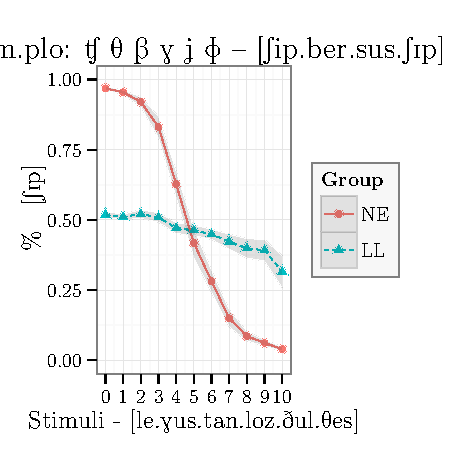
\includegraphics[width=\maxwidth]{figure/ident} 

\end{knitrout}


\begin{figure}
\caption{here is the identification plot}
\centering
% Created by tikzDevice version 0.6.2 on 2013-05-17 11:59:36
% !TEX encoding = UTF-8 Unicode
\begin{tikzpicture}[x=1pt,y=1pt]
\definecolor[named]{drawColor}{rgb}{0.00,0.00,0.00}
\definecolor[named]{fillColor}{rgb}{1.00,1.00,1.00}
\fill[color=fillColor,fill opacity=0.00,] (0,0) rectangle (505.89,505.89);
\begin{scope}
\path[clip] (  0.00,  0.00) rectangle (505.89,505.89);
\end{scope}
\begin{scope}
\path[clip] (  0.00,  0.00) rectangle (505.89,505.89);
\end{scope}
\begin{scope}
\path[clip] (  0.00,  0.00) rectangle (505.89,505.89);
\definecolor[named]{drawColor}{rgb}{1.00,1.00,1.00}
\definecolor[named]{fillColor}{rgb}{1.00,1.00,1.00}

\draw[color=drawColor,line width= 0.6pt,line cap=round,line join=round,fill=fillColor,] (  0.00,  0.00) rectangle (505.89,505.89);
\end{scope}
\begin{scope}
\path[clip] (  0.00,  0.00) rectangle (505.89,505.89);
\end{scope}
\begin{scope}
\path[clip] (  0.00,  0.00) rectangle (505.89,505.89);
\end{scope}
\begin{scope}
\path[clip] (  0.00,  0.00) rectangle (505.89,505.89);
\end{scope}
\begin{scope}
\path[clip] ( 46.54, 36.44) rectangle (429.80,474.29);
\definecolor[named]{fillColor}{rgb}{1.00,1.00,1.00}

\draw[fill=fillColor,draw opacity=0.00,] ( 46.54, 36.44) rectangle (429.80,474.29);
\definecolor[named]{drawColor}{rgb}{0.98,0.98,0.98}

\draw[color=drawColor,line width= 0.6pt,line join=round,fill opacity=0.00,] ( 46.54,106.10) --
	(429.80,106.10);

\draw[color=drawColor,line width= 0.6pt,line join=round,fill opacity=0.00,] ( 46.54,205.61) --
	(429.80,205.61);

\draw[color=drawColor,line width= 0.6pt,line join=round,fill opacity=0.00,] ( 46.54,305.12) --
	(429.80,305.12);

\draw[color=drawColor,line width= 0.6pt,line join=round,fill opacity=0.00,] ( 46.54,404.63) --
	(429.80,404.63);

\draw[color=drawColor,line width= 0.6pt,line join=round,fill opacity=0.00,] ( 46.54, 36.44) --
	( 46.54,474.29);

\draw[color=drawColor,line width= 0.6pt,line join=round,fill opacity=0.00,] ( 81.38, 36.44) --
	( 81.38,474.29);

\draw[color=drawColor,line width= 0.6pt,line join=round,fill opacity=0.00,] (116.22, 36.44) --
	(116.22,474.29);

\draw[color=drawColor,line width= 0.6pt,line join=round,fill opacity=0.00,] (151.07, 36.44) --
	(151.07,474.29);

\draw[color=drawColor,line width= 0.6pt,line join=round,fill opacity=0.00,] (185.91, 36.44) --
	(185.91,474.29);

\draw[color=drawColor,line width= 0.6pt,line join=round,fill opacity=0.00,] (220.75, 36.44) --
	(220.75,474.29);

\draw[color=drawColor,line width= 0.6pt,line join=round,fill opacity=0.00,] (255.59, 36.44) --
	(255.59,474.29);

\draw[color=drawColor,line width= 0.6pt,line join=round,fill opacity=0.00,] (290.43, 36.44) --
	(290.43,474.29);

\draw[color=drawColor,line width= 0.6pt,line join=round,fill opacity=0.00,] (325.28, 36.44) --
	(325.28,474.29);

\draw[color=drawColor,line width= 0.6pt,line join=round,fill opacity=0.00,] (360.12, 36.44) --
	(360.12,474.29);

\draw[color=drawColor,line width= 0.6pt,line join=round,fill opacity=0.00,] (394.96, 36.44) --
	(394.96,474.29);

\draw[color=drawColor,line width= 0.6pt,line join=round,fill opacity=0.00,] (429.80, 36.44) --
	(429.80,474.29);
\definecolor[named]{drawColor}{rgb}{0.90,0.90,0.90}

\draw[color=drawColor,line width= 0.2pt,line join=round,fill opacity=0.00,] ( 46.54, 56.35) --
	(429.80, 56.35);

\draw[color=drawColor,line width= 0.2pt,line join=round,fill opacity=0.00,] ( 46.54,155.86) --
	(429.80,155.86);

\draw[color=drawColor,line width= 0.2pt,line join=round,fill opacity=0.00,] ( 46.54,255.37) --
	(429.80,255.37);

\draw[color=drawColor,line width= 0.2pt,line join=round,fill opacity=0.00,] ( 46.54,354.88) --
	(429.80,354.88);

\draw[color=drawColor,line width= 0.2pt,line join=round,fill opacity=0.00,] ( 46.54,454.39) --
	(429.80,454.39);

\draw[color=drawColor,line width= 0.2pt,line join=round,fill opacity=0.00,] ( 63.96, 36.44) --
	( 63.96,474.29);

\draw[color=drawColor,line width= 0.2pt,line join=round,fill opacity=0.00,] ( 98.80, 36.44) --
	( 98.80,474.29);

\draw[color=drawColor,line width= 0.2pt,line join=round,fill opacity=0.00,] (133.64, 36.44) --
	(133.64,474.29);

\draw[color=drawColor,line width= 0.2pt,line join=round,fill opacity=0.00,] (168.49, 36.44) --
	(168.49,474.29);

\draw[color=drawColor,line width= 0.2pt,line join=round,fill opacity=0.00,] (203.33, 36.44) --
	(203.33,474.29);

\draw[color=drawColor,line width= 0.2pt,line join=round,fill opacity=0.00,] (238.17, 36.44) --
	(238.17,474.29);

\draw[color=drawColor,line width= 0.2pt,line join=round,fill opacity=0.00,] (273.01, 36.44) --
	(273.01,474.29);

\draw[color=drawColor,line width= 0.2pt,line join=round,fill opacity=0.00,] (307.86, 36.44) --
	(307.86,474.29);

\draw[color=drawColor,line width= 0.2pt,line join=round,fill opacity=0.00,] (342.70, 36.44) --
	(342.70,474.29);

\draw[color=drawColor,line width= 0.2pt,line join=round,fill opacity=0.00,] (377.54, 36.44) --
	(377.54,474.29);

\draw[color=drawColor,line width= 0.2pt,line join=round,fill opacity=0.00,] (412.38, 36.44) --
	(412.38,474.29);
\definecolor[named]{drawColor}{rgb}{0.97,0.46,0.43}
\definecolor[named]{fillColor}{rgb}{0.97,0.46,0.43}

\draw[color=drawColor,line width= 0.5pt,line join=round,] ( 63.96,442.05) --
	( 98.80,436.48) --
	(133.64,422.94) --
	(168.49,387.12) --
	(203.33,306.32) --
	(238.17,222.73) --
	(273.01,168.59) --
	(307.86,116.05) --
	(342.70, 90.58) --
	(377.54, 81.02) --
	(412.38, 72.27);
\definecolor[named]{drawColor}{rgb}{0.00,0.75,0.77}
\definecolor[named]{fillColor}{rgb}{0.00,0.75,0.77}

\draw[color=drawColor,line width= 0.5pt,dash pattern=on 2pt off 2pt ,line join=round,] ( 63.96,262.93) --
	( 98.80,259.75) --
	(133.64,263.73) --
	(168.49,258.95) --
	(203.33,243.82) --
	(238.17,240.64) --
	(273.01,235.07) --
	(307.86,224.72) --
	(342.70,215.17) --
	(377.54,212.38) --
	(412.38,182.13);
\definecolor[named]{fillColor}{rgb}{0.97,0.46,0.43}

\draw[fill=fillColor,draw opacity=0.00,] ( 63.96,442.05) circle (  2.13);
\definecolor[named]{fillColor}{rgb}{0.00,0.75,0.77}

\draw[fill=fillColor,draw opacity=0.00,] ( 63.96,266.25) --
	( 66.83,261.27) --
	( 61.09,261.27) --
	cycle;
\definecolor[named]{fillColor}{rgb}{0.97,0.46,0.43}

\draw[fill=fillColor,draw opacity=0.00,] ( 98.80,436.48) circle (  2.13);
\definecolor[named]{fillColor}{rgb}{0.00,0.75,0.77}

\draw[fill=fillColor,draw opacity=0.00,] ( 98.80,263.06) --
	(101.68,258.09) --
	( 95.93,258.09) --
	cycle;
\definecolor[named]{fillColor}{rgb}{0.97,0.46,0.43}

\draw[fill=fillColor,draw opacity=0.00,] (133.64,422.94) circle (  2.13);
\definecolor[named]{fillColor}{rgb}{0.00,0.75,0.77}

\draw[fill=fillColor,draw opacity=0.00,] (133.64,267.04) --
	(136.52,262.07) --
	(130.77,262.07) --
	cycle;
\definecolor[named]{fillColor}{rgb}{0.97,0.46,0.43}

\draw[fill=fillColor,draw opacity=0.00,] (168.49,387.12) circle (  2.13);
\definecolor[named]{fillColor}{rgb}{0.00,0.75,0.77}

\draw[fill=fillColor,draw opacity=0.00,] (168.49,262.27) --
	(171.36,257.29) --
	(165.61,257.29) --
	cycle;
\definecolor[named]{fillColor}{rgb}{0.97,0.46,0.43}

\draw[fill=fillColor,draw opacity=0.00,] (203.33,306.32) circle (  2.13);
\definecolor[named]{fillColor}{rgb}{0.00,0.75,0.77}

\draw[fill=fillColor,draw opacity=0.00,] (203.33,247.14) --
	(206.20,242.16) --
	(200.46,242.16) --
	cycle;
\definecolor[named]{fillColor}{rgb}{0.97,0.46,0.43}

\draw[fill=fillColor,draw opacity=0.00,] (238.17,222.73) circle (  2.13);
\definecolor[named]{fillColor}{rgb}{0.00,0.75,0.77}

\draw[fill=fillColor,draw opacity=0.00,] (238.17,243.96) --
	(241.05,238.98) --
	(235.30,238.98) --
	cycle;
\definecolor[named]{fillColor}{rgb}{0.97,0.46,0.43}

\draw[fill=fillColor,draw opacity=0.00,] (273.01,168.59) circle (  2.13);
\definecolor[named]{fillColor}{rgb}{0.00,0.75,0.77}

\draw[fill=fillColor,draw opacity=0.00,] (273.01,238.39) --
	(275.89,233.41) --
	(270.14,233.41) --
	cycle;
\definecolor[named]{fillColor}{rgb}{0.97,0.46,0.43}

\draw[fill=fillColor,draw opacity=0.00,] (307.86,116.05) circle (  2.13);
\definecolor[named]{fillColor}{rgb}{0.00,0.75,0.77}

\draw[fill=fillColor,draw opacity=0.00,] (307.86,228.04) --
	(310.73,223.06) --
	(304.98,223.06) --
	cycle;
\definecolor[named]{fillColor}{rgb}{0.97,0.46,0.43}

\draw[fill=fillColor,draw opacity=0.00,] (342.70, 90.58) circle (  2.13);
\definecolor[named]{fillColor}{rgb}{0.00,0.75,0.77}

\draw[fill=fillColor,draw opacity=0.00,] (342.70,218.48) --
	(345.57,213.51) --
	(339.82,213.51) --
	cycle;
\definecolor[named]{fillColor}{rgb}{0.97,0.46,0.43}

\draw[fill=fillColor,draw opacity=0.00,] (377.54, 81.02) circle (  2.13);
\definecolor[named]{fillColor}{rgb}{0.00,0.75,0.77}

\draw[fill=fillColor,draw opacity=0.00,] (377.54,215.70) --
	(380.41,210.72) --
	(374.67,210.72) --
	cycle;
\definecolor[named]{fillColor}{rgb}{0.97,0.46,0.43}

\draw[fill=fillColor,draw opacity=0.00,] (412.38, 72.27) circle (  2.13);
\definecolor[named]{fillColor}{rgb}{0.00,0.75,0.77}

\draw[fill=fillColor,draw opacity=0.00,] (412.38,185.45) --
	(415.26,180.47) --
	(409.51,180.47) --
	cycle;
\definecolor[named]{fillColor}{rgb}{0.20,0.20,0.20}

\draw[fill=fillColor,fill opacity=0.15,draw opacity=0.00,] ( 63.96,444.80) --
	( 98.80,439.34) --
	(133.64,429.75) --
	(168.49,401.82) --
	(203.33,324.69) --
	(238.17,243.22) --
	(273.01,184.13) --
	(307.86,127.93) --
	(342.70, 97.14) --
	(377.54, 85.38) --
	(412.38, 75.23) --
	(412.38, 69.30) --
	(377.54, 76.67) --
	(342.70, 84.02) --
	(307.86,104.17) --
	(273.01,153.06) --
	(238.17,202.23) --
	(203.33,287.94) --
	(168.49,372.42) --
	(133.64,416.14) --
	( 98.80,433.62) --
	( 63.96,439.30) --
	cycle;

\draw[fill=fillColor,fill opacity=0.15,draw opacity=0.00,] ( 63.96,267.06) --
	( 98.80,263.70) --
	(133.64,269.79) --
	(168.49,265.54) --
	(203.33,251.36) --
	(238.17,247.98) --
	(273.01,242.25) --
	(307.86,235.17) --
	(342.70,228.97) --
	(377.54,227.48) --
	(412.38,204.39) --
	(412.38,159.87) --
	(377.54,197.28) --
	(342.70,201.36) --
	(307.86,214.27) --
	(273.01,227.89) --
	(238.17,233.30) --
	(203.33,236.28) --
	(168.49,252.36) --
	(133.64,257.66) --
	( 98.80,255.79) --
	( 63.96,258.80) --
	cycle;
\definecolor[named]{drawColor}{rgb}{0.50,0.50,0.50}

\draw[color=drawColor,line width= 0.6pt,line cap=round,line join=round,fill opacity=0.00,] ( 46.54, 36.44) rectangle (429.80,474.29);
\end{scope}
\begin{scope}
\path[clip] (  0.00,  0.00) rectangle (505.89,505.89);
\end{scope}
\begin{scope}
\path[clip] (  0.00,  0.00) rectangle (505.89,505.89);
\end{scope}
\begin{scope}
\path[clip] (  0.00,  0.00) rectangle (505.89,505.89);
\definecolor[named]{drawColor}{rgb}{0.00,0.00,0.00}

\node[color=drawColor,anchor=base east,inner sep=0pt, outer sep=0pt, scale=  0.80] at ( 39.43, 53.04) {0.00};

\node[color=drawColor,anchor=base east,inner sep=0pt, outer sep=0pt, scale=  0.80] at ( 39.43,152.55) {0.25};

\node[color=drawColor,anchor=base east,inner sep=0pt, outer sep=0pt, scale=  0.80] at ( 39.43,252.06) {0.50};

\node[color=drawColor,anchor=base east,inner sep=0pt, outer sep=0pt, scale=  0.80] at ( 39.43,351.57) {0.75};

\node[color=drawColor,anchor=base east,inner sep=0pt, outer sep=0pt, scale=  0.80] at ( 39.43,451.08) {1.00};
\end{scope}
\begin{scope}
\path[clip] (  0.00,  0.00) rectangle (505.89,505.89);
\end{scope}
\begin{scope}
\path[clip] (  0.00,  0.00) rectangle (505.89,505.89);
\definecolor[named]{drawColor}{rgb}{0.00,0.00,0.00}

\draw[color=drawColor,line width= 0.6pt,line join=round,fill opacity=0.00,] ( 42.27, 56.35) --
	( 46.54, 56.35);

\draw[color=drawColor,line width= 0.6pt,line join=round,fill opacity=0.00,] ( 42.27,155.86) --
	( 46.54,155.86);

\draw[color=drawColor,line width= 0.6pt,line join=round,fill opacity=0.00,] ( 42.27,255.37) --
	( 46.54,255.37);

\draw[color=drawColor,line width= 0.6pt,line join=round,fill opacity=0.00,] ( 42.27,354.88) --
	( 46.54,354.88);

\draw[color=drawColor,line width= 0.6pt,line join=round,fill opacity=0.00,] ( 42.27,454.39) --
	( 46.54,454.39);
\end{scope}
\begin{scope}
\path[clip] (  0.00,  0.00) rectangle (505.89,505.89);
\end{scope}
\begin{scope}
\path[clip] (  0.00,  0.00) rectangle (505.89,505.89);
\end{scope}
\begin{scope}
\path[clip] (  0.00,  0.00) rectangle (505.89,505.89);
\end{scope}
\begin{scope}
\path[clip] (  0.00,  0.00) rectangle (505.89,505.89);
\end{scope}
\begin{scope}
\path[clip] (  0.00,  0.00) rectangle (505.89,505.89);
\end{scope}
\begin{scope}
\path[clip] (  0.00,  0.00) rectangle (505.89,505.89);
\definecolor[named]{drawColor}{rgb}{0.00,0.00,0.00}

\draw[color=drawColor,line width= 0.6pt,line join=round,fill opacity=0.00,] ( 63.96, 32.18) --
	( 63.96, 36.44);

\draw[color=drawColor,line width= 0.6pt,line join=round,fill opacity=0.00,] ( 98.80, 32.18) --
	( 98.80, 36.44);

\draw[color=drawColor,line width= 0.6pt,line join=round,fill opacity=0.00,] (133.64, 32.18) --
	(133.64, 36.44);

\draw[color=drawColor,line width= 0.6pt,line join=round,fill opacity=0.00,] (168.49, 32.18) --
	(168.49, 36.44);

\draw[color=drawColor,line width= 0.6pt,line join=round,fill opacity=0.00,] (203.33, 32.18) --
	(203.33, 36.44);

\draw[color=drawColor,line width= 0.6pt,line join=round,fill opacity=0.00,] (238.17, 32.18) --
	(238.17, 36.44);

\draw[color=drawColor,line width= 0.6pt,line join=round,fill opacity=0.00,] (273.01, 32.18) --
	(273.01, 36.44);

\draw[color=drawColor,line width= 0.6pt,line join=round,fill opacity=0.00,] (307.86, 32.18) --
	(307.86, 36.44);

\draw[color=drawColor,line width= 0.6pt,line join=round,fill opacity=0.00,] (342.70, 32.18) --
	(342.70, 36.44);

\draw[color=drawColor,line width= 0.6pt,line join=round,fill opacity=0.00,] (377.54, 32.18) --
	(377.54, 36.44);

\draw[color=drawColor,line width= 0.6pt,line join=round,fill opacity=0.00,] (412.38, 32.18) --
	(412.38, 36.44);
\end{scope}
\begin{scope}
\path[clip] (  0.00,  0.00) rectangle (505.89,505.89);
\end{scope}
\begin{scope}
\path[clip] (  0.00,  0.00) rectangle (505.89,505.89);
\definecolor[named]{drawColor}{rgb}{0.00,0.00,0.00}

\node[color=drawColor,anchor=base,inner sep=0pt, outer sep=0pt, scale=  0.80] at ( 63.96, 22.72) {0};

\node[color=drawColor,anchor=base,inner sep=0pt, outer sep=0pt, scale=  0.80] at ( 98.80, 22.72) {1};

\node[color=drawColor,anchor=base,inner sep=0pt, outer sep=0pt, scale=  0.80] at (133.64, 22.72) {2};

\node[color=drawColor,anchor=base,inner sep=0pt, outer sep=0pt, scale=  0.80] at (168.49, 22.72) {3};

\node[color=drawColor,anchor=base,inner sep=0pt, outer sep=0pt, scale=  0.80] at (203.33, 22.72) {4};

\node[color=drawColor,anchor=base,inner sep=0pt, outer sep=0pt, scale=  0.80] at (238.17, 22.72) {5};

\node[color=drawColor,anchor=base,inner sep=0pt, outer sep=0pt, scale=  0.80] at (273.01, 22.72) {6};

\node[color=drawColor,anchor=base,inner sep=0pt, outer sep=0pt, scale=  0.80] at (307.86, 22.72) {7};

\node[color=drawColor,anchor=base,inner sep=0pt, outer sep=0pt, scale=  0.80] at (342.70, 22.72) {8};

\node[color=drawColor,anchor=base,inner sep=0pt, outer sep=0pt, scale=  0.80] at (377.54, 22.72) {9};

\node[color=drawColor,anchor=base,inner sep=0pt, outer sep=0pt, scale=  0.80] at (412.38, 22.72) {10};
\end{scope}
\begin{scope}
\path[clip] (  0.00,  0.00) rectangle (505.89,505.89);
\end{scope}
\begin{scope}
\path[clip] (  0.00,  0.00) rectangle (505.89,505.89);
\end{scope}
\begin{scope}
\path[clip] (  0.00,  0.00) rectangle (505.89,505.89);
\end{scope}
\begin{scope}
\path[clip] (  0.00,  0.00) rectangle (505.89,505.89);
\end{scope}
\begin{scope}
\path[clip] (  0.00,  0.00) rectangle (505.89,505.89);
\definecolor[named]{drawColor}{rgb}{0.00,0.00,0.00}

\node[color=drawColor,anchor=base,inner sep=0pt, outer sep=0pt, scale=  1.00] at (238.17, 10.84) {Stimuli - [le.\textgamma us.tan.loz.\textipa{D}ul.\texttheta es]};
\end{scope}
\begin{scope}
\path[clip] (  0.00,  0.00) rectangle (505.89,505.89);
\end{scope}
\begin{scope}
\path[clip] (  0.00,  0.00) rectangle (505.89,505.89);
\definecolor[named]{drawColor}{rgb}{0.00,0.00,0.00}

\node[rotate= 90.00,color=drawColor,anchor=base,inner sep=0pt, outer sep=0pt, scale=  1.00] at ( 19.11,255.37) {\ \ \ \% \ \ [\textesh\textsci p]};
\end{scope}
\begin{scope}
\path[clip] (  0.00,  0.00) rectangle (505.89,505.89);
\end{scope}
\begin{scope}
\path[clip] (  0.00,  0.00) rectangle (505.89,505.89);
\end{scope}
\begin{scope}
\path[clip] (  0.00,  0.00) rectangle (505.89,505.89);
\end{scope}
\begin{scope}
\path[clip] (  0.00,  0.00) rectangle (505.89,505.89);
\end{scope}
\begin{scope}
\path[clip] (  0.00,  0.00) rectangle (505.89,505.89);
\end{scope}
\begin{scope}
\path[clip] (  0.00,  0.00) rectangle (505.89,505.89);
\definecolor[named]{drawColor}{rgb}{0.50,0.50,0.50}
\definecolor[named]{fillColor}{rgb}{0.97,0.97,0.97}

\draw[color=drawColor,line width= 0.7pt,line cap=round,line join=round,fill=fillColor,] (439.88,228.27) rectangle (481.36,282.46);
\end{scope}
\begin{scope}
\path[clip] (  0.00,  0.00) rectangle (505.89,505.89);
\end{scope}
\begin{scope}
\path[clip] (  0.00,  0.00) rectangle (505.89,505.89);
\definecolor[named]{drawColor}{rgb}{0.00,0.00,0.00}

\node[color=drawColor,anchor=base west,inner sep=0pt, outer sep=0pt, scale=  0.80] at (444.14,271.57) {\bfseries Group};
\end{scope}
\begin{scope}
\path[clip] (  0.00,  0.00) rectangle (505.89,505.89);
\end{scope}
\begin{scope}
\path[clip] (  0.00,  0.00) rectangle (505.89,505.89);
\definecolor[named]{drawColor}{rgb}{0.80,0.80,0.80}
\definecolor[named]{fillColor}{rgb}{1.00,1.00,1.00}

\draw[color=drawColor,line width= 0.6pt,line cap=round,line join=round,fill=fillColor,] (444.14,249.89) rectangle (461.49,267.23);
\end{scope}
\begin{scope}
\path[clip] (  0.00,  0.00) rectangle (505.89,505.89);
\end{scope}
\begin{scope}
\path[clip] (  0.00,  0.00) rectangle (505.89,505.89);
\definecolor[named]{drawColor}{rgb}{0.97,0.46,0.43}

\draw[color=drawColor,line width= 0.5pt,line join=round,fill opacity=0.00,] (445.88,258.56) -- (459.75,258.56);
\end{scope}
\begin{scope}
\path[clip] (  0.00,  0.00) rectangle (505.89,505.89);
\end{scope}
\begin{scope}
\path[clip] (  0.00,  0.00) rectangle (505.89,505.89);
\definecolor[named]{fillColor}{rgb}{0.97,0.46,0.43}

\draw[fill=fillColor,draw opacity=0.00,] (452.82,258.56) circle (  2.13);
\end{scope}
\begin{scope}
\path[clip] (  0.00,  0.00) rectangle (505.89,505.89);
\end{scope}
\begin{scope}
\path[clip] (  0.00,  0.00) rectangle (505.89,505.89);
\definecolor[named]{fillColor}{rgb}{0.20,0.20,0.20}

\draw[fill=fillColor,fill opacity=0.15,draw opacity=0.00,] (444.14,249.89) rectangle (461.49,267.23);
\end{scope}
\begin{scope}
\path[clip] (  0.00,  0.00) rectangle (505.89,505.89);
\end{scope}
\begin{scope}
\path[clip] (  0.00,  0.00) rectangle (505.89,505.89);
\definecolor[named]{drawColor}{rgb}{0.80,0.80,0.80}
\definecolor[named]{fillColor}{rgb}{1.00,1.00,1.00}

\draw[color=drawColor,line width= 0.6pt,line cap=round,line join=round,fill=fillColor,] (444.14,232.54) rectangle (461.49,249.89);
\end{scope}
\begin{scope}
\path[clip] (  0.00,  0.00) rectangle (505.89,505.89);
\end{scope}
\begin{scope}
\path[clip] (  0.00,  0.00) rectangle (505.89,505.89);
\definecolor[named]{drawColor}{rgb}{0.00,0.75,0.77}

\draw[color=drawColor,line width= 0.5pt,dash pattern=on 2pt off 2pt ,line join=round,fill opacity=0.00,] (445.88,241.21) -- (459.75,241.21);
\end{scope}
\begin{scope}
\path[clip] (  0.00,  0.00) rectangle (505.89,505.89);
\end{scope}
\begin{scope}
\path[clip] (  0.00,  0.00) rectangle (505.89,505.89);
\definecolor[named]{fillColor}{rgb}{0.00,0.75,0.77}

\draw[fill=fillColor,draw opacity=0.00,] (452.82,244.53) --
	(455.69,239.56) --
	(449.94,239.56) --
	cycle;
\end{scope}
\begin{scope}
\path[clip] (  0.00,  0.00) rectangle (505.89,505.89);
\end{scope}
\begin{scope}
\path[clip] (  0.00,  0.00) rectangle (505.89,505.89);
\definecolor[named]{fillColor}{rgb}{0.20,0.20,0.20}

\draw[fill=fillColor,fill opacity=0.15,draw opacity=0.00,] (444.14,232.54) rectangle (461.49,249.89);
\end{scope}
\begin{scope}
\path[clip] (  0.00,  0.00) rectangle (505.89,505.89);
\end{scope}
\begin{scope}
\path[clip] (  0.00,  0.00) rectangle (505.89,505.89);
\definecolor[named]{drawColor}{rgb}{0.00,0.00,0.00}

\node[color=drawColor,anchor=base west,inner sep=0pt, outer sep=0pt, scale=  0.80] at (463.66,255.25) {NE};
\end{scope}
\begin{scope}
\path[clip] (  0.00,  0.00) rectangle (505.89,505.89);
\end{scope}
\begin{scope}
\path[clip] (  0.00,  0.00) rectangle (505.89,505.89);
\definecolor[named]{drawColor}{rgb}{0.00,0.00,0.00}

\node[color=drawColor,anchor=base west,inner sep=0pt, outer sep=0pt, scale=  0.80] at (463.66,237.91) {LL};
\end{scope}
\begin{scope}
\path[clip] (  0.00,  0.00) rectangle (505.89,505.89);
\end{scope}
\begin{scope}
\path[clip] (  0.00,  0.00) rectangle (505.89,505.89);
\end{scope}
\begin{scope}
\path[clip] (  0.00,  0.00) rectangle (505.89,505.89);
\end{scope}
\begin{scope}
\path[clip] (  0.00,  0.00) rectangle (505.89,505.89);
\end{scope}
\begin{scope}
\path[clip] (  0.00,  0.00) rectangle (505.89,505.89);
\end{scope}
\begin{scope}
\path[clip] (  0.00,  0.00) rectangle (505.89,505.89);
\end{scope}
\begin{scope}
\path[clip] (  0.00,  0.00) rectangle (505.89,505.89);
\end{scope}
\begin{scope}
\path[clip] (  0.00,  0.00) rectangle (505.89,505.89);
\end{scope}
\begin{scope}
\path[clip] (  0.00,  0.00) rectangle (505.89,505.89);
\end{scope}
\begin{scope}
\path[clip] (  0.00,  0.00) rectangle (505.89,505.89);
\definecolor[named]{drawColor}{rgb}{0.00,0.00,0.00}

\node[color=drawColor,anchor=base,inner sep=0pt, outer sep=0pt, scale=  1.20] at (238.17,477.90) {e.xem.plo: \textteshlig \ \texttheta \ \textbeta \ \textgamma \ \textctj \ \textipa{F} -- [\textesh ip.be\textipa{r}.sus.\textesh\textsci p]};
\end{scope}
\begin{scope}
\path[clip] (  0.00,  0.00) rectangle (505.89,505.89);
\end{scope}
\begin{scope}
\path[clip] (  0.00,  0.00) rectangle (505.89,505.89);
\end{scope}
\end{tikzpicture}

\end{figure}

% section ident_example (end)

\end{document}

